\documentclass[11pt,a4paper]{article}
\usepackage{gtu-el-yazisi}
\begin{document}
\notbilgi{Nümerik Analiz}{7. Ders -- Nümerik Diferansiyelleme}{Numerik-7.ders.pdf}

\sayfa{1}
\section{Nümerik Diferansiyelleme}
\noindent\underline{\small iki nokta formülü}
\[
  f'(x_0) = \lim_{h\to 0}\frac{f(x_0+h) - f(x_0)}{h}
\]
\begin{center}
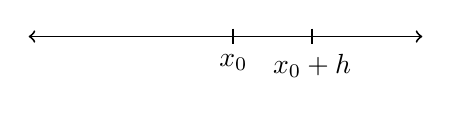
\begin{tikzpicture}[line width=0.7pt]
  \draw[<->] (0,0) -- (5,0);
  \draw (2.6,0.1) -- (2.6,-0.1) node[below] {$x_0$};
  \draw (3.6,0.1) -- (3.6,-0.1) node[below] {$x_0+h$};
\end{tikzpicture}
\end{center}
\[
  f'(x_0) \approx \frac{f(x_0+h) - f(x_0)}{h}
\]
$f \in C^2[a,b]$ bir fonk, \quad $x_0 \in (a,b)$ bir nokta\\
\fbox{$x_1 = x_0 + h$} $\in [a,b]$ olacak şekilde bir $h$ alalım.
\[
  \begin{array}{c|c}
    x & f(x)\\ \hline
    x_0 & f(x_0)\\
    x_1 & f(x_1)
  \end{array}
  \;\Bigg\}\quad
  \underbrace{L_{1,0}(x)}_{\frac{x-x_1}{x_0-x_1}}f(x_0) + \underbrace{L_{1,1}(x)}_{\frac{x-x_0}{x_1-x_0}}f(x_1) = P_1(x)
\]
\begin{align*}
  P_1(x) &= \frac{x - x_0 - h}{-h}\,f(x_0) + \frac{x - x_0}{h}\,f(x_0+h),\\
  f(x) &= P_1(x) + f''(\xi)\,(x-x_0)(x-x_0-h)\footnotemark\\
  P_1'(x) &= \frac{-f(x_0)}{h} + \frac{f(x_0+h)}{h} \approx f'(x_0)\\
  f'(x) &= \frac{f(x_0+h) - f(x_0)}{h} + \frac{2(x-x_0) - h}{2}\,f''(\xi)
           + \left(\frac{f''(\xi)}{2}\right)'_x (x-x_0)(x-x_0-h)
\end{align*}
\footnotetext{Claude notu: muhtemelen $\frac{f''(\xi)}{2}$ olmalı (bir sonraki satırda $/2$ var).}
\[
  f'(x_0) = P_1'(x_0) - \underbrace{\frac{h}{2}\,f''(\xi)}_{} \qquad x_0 \le \xi \le x_0 + h
\]

\noindent\vurgu{Not 1} \ $f(x)$'in $x_0$ noktasından \textsuperscript{hata terimli} Taylor formülü
\[
  f(x) = f(x_0) + f'(x_0)(x-x_0) + \frac{f''(\xi)}{2!}(x-x_0)^2, \quad \xi \in (x_0, x)
\]
$x = x_0 + h$ yazalım
\begin{align*}
  f(x_0+h) &= f(x_0) + f'(x_0)(x_0+h-x_0) + \frac{f''(\xi)}{2}(x_0+h-x_0)^2\\
           &= f(x_0) + f'(x_0)\,h + h^2\,\frac{f''(\xi)}{2} \qquad \xi \in (x_0, x_0+h)
\end{align*}
\[
  f'(x) = \frac{f(x_0+h) - f(x_0)}{h} - h\,\frac{f''(\xi)}{2} \qquad \xi \in (x_0, x_0+h)
\]

\sayfa{2}
\begin{ornek}[1]
\begin{center}
\begin{tabular}{r|c|c|c|c}
 & $x$ & $f(x)$ & $f'(x)$ & $f'(x)$ geri\\ \hline
ileri $\rightarrow$ & $0{,}5$ & \okunamadi{0,48} & $0{,}8$ & \\
ileri / geri $\rightarrow$ & $0{,}6$ & $0{,}56$ & $1$ & $0{,}8$\\
geri $\rightarrow$ & $0{,}7$ & $0{,}66$ & & $1$
\end{tabular}
\end{center}
{\small(Sol kenarda ardışık satırlar arasında ``$0{,}1$'' adım işaretleri.)}

geri fark tüm ileri fark formüllerinde $h \Rightarrow -h$ konularak bulunur.
\end{ornek}

\begin{ornek}[2]
$f(x) = \ln x$, \ $x_0 = 1{,}8$ noktasında 1. mertebeden türevi $h = 0{,}01$ olacak biçimde
tahmini hesaplayıp hatasını değerlendiriniz.
\end{ornek}
\[
  f'(1{,}8) = \frac{f(1{,}8 + 0{,}01) - f(1{,}8)}{0{,}01} = \frac{\ln(1{,}81) - \ln(1{,}8)}{0{,}01}
  = 0{,}5540
\]
\begin{align*}
  R(1{,}8) &= -\frac{h}{2}\,f''(\xi) \qquad \xi \in (1{,}8;\ 1{,}81)
  \qquad\qquad f(x) = \ln x,\ f'(x) = \frac{1}{x},\ f''(x) = -\frac{1}{x^2}\\
  &= \left|\frac{h^2}{2}\cdot\frac{1}{\xi^2}\right|\footnotemark = \left|\frac{0{,}01}{2}\cdot\frac{1}{\xi^2}\right|\\
  &\le \frac{0{,}01}{2}\cdot\frac{1}{(1{,}8)^2} \le 1{,}5\cdot10^{-3}
\end{align*}
\footnotetext{Claude notu: muhtemelen $\frac{h}{2}$ olmalı (hata terimi $-\frac{h}{2}f''(\xi)$; sonraki adımda da $\frac{0{,}01}{2}$ kullanılmış).}
\[
  0{,}5525 \le f'(1{,}8) \le 0{,}5555
\]
\[
  \frac{1}{1{,}8} \approx 0{,}5555
\]

\sayfa{3}
$f \in C^3[a,b]$ ve $x_0 \in (a,b)$, $h \ne 0$ adımı ile\\
\hspace*{1.5em}$x_1 = x_0 + h$, \ $x_2 = x_0 + 2h \in [a,b]$ tanımlansın

\noindent
\begin{minipage}[c]{0.6\linewidth}
\begin{align*}
  P_2(x) &= L_{2,0}(x)\,f(x_0) + L_{2,1}(x)\,f(x_1) + L_{2,2}(x)\,f(x_2)\\
  L_{2,0}(x) &= \frac{(x-x_1)(x-x_2)}{(x_0-x_1)(x_0-x_2)}\\
  L_{2,1}(x) &= \frac{(x-x_0)(x-x_2)}{(x_1-x_0)(x_1-x_2)}\\
  L_{2,2}(x) &= \frac{(x-x_0)(x-x_1)}{(x_2-x_0)(x_2-x_1)}
\end{align*}
\end{minipage}\hfill
\begin{minipage}[c]{0.36\linewidth}
\centering
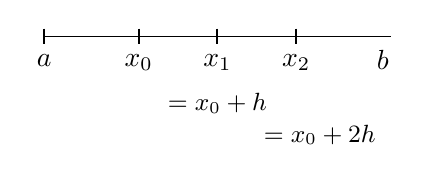
\begin{tikzpicture}[line width=0.7pt]
  \draw (0,0) -- (4.4,0);
  \foreach \x/\n in {0/a,1.2/x_0,2.2/x_1,3.2/x_2}{
    \draw (\x,0.1) -- (\x,-0.1) node[below] {$\n$};}
  \node[below] at (4.3,-0.05) {$b$};
  \node[font=\small] at (2.2,-0.85) {$=x_0+h$};
  \node[font=\small] at (3.5,-1.25) {$=x_0+2h$};
\end{tikzpicture}
\end{minipage}

\begin{align*}
  f(x) &= P_2(x) + \frac{f'''(\xi)}{3!}(x-x_0)(x-x_1)(x-x_2)\\
  f'(x) &= P_2'(x) + \left(\frac{f'''(\xi)}{3!}\right)'_x (x-x_0)(x-x_0-h)(x-x_0-2h)\\
  &\quad + \frac{f'''(\xi)}{6}\Big[(x-x_0-h)(x-x_0-2h) + (x-x_0)(x-x_0-2h)\\
  &\qquad\qquad\qquad + (x-x_0)(x-x_0-h)\Big]\\
  P_2'(x) &= \frac{2x - (2x_0+3h)}{2h^2}\,f(x_0) + \frac{2x - (2x_0+2h)}{-h^2}\,f(x_0+h)\\
  &\quad + \frac{2x - (2x_0+h)}{2h^2}\,f(x_0+2h)
\end{align*}
\[
  \hookrightarrow\quad f'(x_0) = P_2'(x_0) + \frac{f'''(\xi)}{6}\,2h^2 \qquad x_0 < \xi < x_0 + 2h
\]

\subsection{3 nokta (üç nokta) formülü}
\[
  \bigstar\quad P_2'(x_0) = \frac{1}{2h}\Big[-3f(x_0) + 4f(x_0+h) - f(x_0+2h)\Big] \approx f'(x_0)
\]
Türevde $x = x_1 = x_0 + h$

\noindent
\begin{minipage}[c]{0.68\linewidth}
\[
  \left.
  \begin{aligned}
    f'(x_0+h) &= P_2'(x_0+h) + \frac{f'''(\xi)}{6}(-h^2)\\
    P_2'(x_0+h) &= \frac{1}{2h}\Big[-f(x_0) + f(x_0+2h)\Big]
  \end{aligned}
  \right\}
\]
\end{minipage}\hfill
\begin{minipage}[c]{0.3\linewidth}
\centering
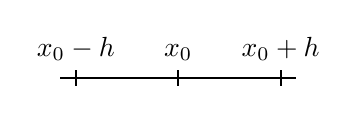
\begin{tikzpicture}[line width=0.7pt]
  \draw (0,0) -- (3,0);
  \foreach \x/\n in {0.2/x_0-h,1.5/x_0,2.8/x_0+h}{
    \draw (\x,0.1) -- (\x,-0.1) node[above=2mm] {$\n$};}
\end{tikzpicture}
\end{minipage}
\[
  \swarrow\quad f'(x_0) = \frac{1}{2h}\Big[f(x_0+h) - f(x_0-h)\Big] - \frac{h^2}{6}\,f'''(\xi)
\]
\[
  x_0 - h < \xi < x_0 + h
\]
\begin{center}
\begin{tikzpicture}[line width=0.7pt, scale=1.2]
  \draw[domain=-1.15:1.15, samples=40, smooth] plot (\x, {1 - 0.85*\x*\x});
  \draw (-1.1,1) -- (1.1,1);
  \draw (-1,0.15) -- (1,0.15);
  \draw[kursunkalem, line width=0.4pt] (-1,0.15) -- (0,1) -- (1,0.15);
  \fill (-1,0.15) circle (1.5pt) (0,1) circle (1.5pt) (1,0.15) circle (1.5pt);
\end{tikzpicture}
\end{center}

\sayfa{4}
{\small\color{kursunkalem}(Bu sayfa çok silik kurşun kalemle yazılmış; tablo değerleri zor okunuyor.)}

\begin{ornek}[3]
\noindent
\begin{minipage}[t]{0.45\linewidth}
\centering
\begin{tabular}{c|c|c}
$x$ & $f(x)$ & $f'(x)$\\ \hline
$1{,}9$ & \okunamadi{13,5} & \\
$2{,}0$ & \okunamadi{11,3} & $?$\\
$2{,}1$ & \okunamadi{13,7} & \\
$2{,}2$ & \okunamadi{13,7} &
\end{tabular}
\quad $6{,}5$
\end{minipage}\hfill
\begin{minipage}[t]{0.5\linewidth}
$f'(x)$: $2{,}0$'daki değeri? tahmin ediniz
\end{minipage}

\elcizimi[0.7]{sekiller/Numerik-7.ders-s4-1.png}[4]
\end{ornek}

\subsection{2. mertebeden türev için nümerik diferansiyelleme formülü}
$f \in C^4[a,b]$ ve $x_0 \in (a,b)$ verilmiş, $x = x_0$ noktasındaki Taylor formülüne göre
\begin{align*}
  f(x) &= f(x_0) + f'(x_0)(x-x_0) + \frac{f''(x_0)}{2!}(x-x_0)^2 + \frac{f'''(x_0)}{3!}(x-x_0)^3\\
       &\quad + \frac{f^{(4)}(\xi)}{4!}(x-x_0)^4
\end{align*}
\begin{align*}
  f(x_0+h) &= f(x_0) + f'(x_0)h + \frac{f''(x_0)}{2!}h^2 + \frac{f'''(x_0)}{3!}h^3
              + \frac{f^{(4)}(\xi_1)}{4!}h^4\\
  f(x_0-h) &= f(x_0) - f'(x_0)h + \frac{f''(x_0)}{2!}h^2 - \frac{f'''(x_0)}{3!}h^3
              + \frac{f^{(4)}(\xi_2)}{4!}h^4
\end{align*}
\[
  f(x_0+h) - f(x_0-h) = f'(x_0)\,2h + f'''(\xi)\,2h^3
\]
\begin{center}
(midpoint'a: $2h$'a bölersek benzer\okunamadi{i})
\end{center}
{\small(Solda ``ikisini toplayalım'' notu; iki açılımdan aşağıdaki toplama ok.)}
\[
  f(x_0+h) + f(x_0-h) = 2f(x_0) + 2\,\frac{f''(x_0)}{2!}h^2
  + \underbrace{\frac{f^{(4)}(\xi_1)}{4!}h^4 + \frac{f^{(4)}(\xi_2)}{4!}h^4}_{\displaystyle\rightarrow\ \frac{f^{(4)}(\xi_1) + f^{(4)}(\xi_2)}{2} = f^{(4)}(\xi)}
\]
\[
  \Leftrightarrow
\]
\[
  \rightarrow\quad f''(x_0) = \frac{f(x_0-h) - 2f(x_0) + f(x_0+h)}{h^2}
  - \underbrace{\frac{h^2}{12}\,f^{(4)}(\xi)}_{\text{hata}}
\]

\sayfa{5}
\begin{ornek}[4]
$f(x) = xe^x \rightarrow f''(2)$'yi tahmin edin ve hatasını belirtin\\
$h_1 = 0{,}1$ \qquad $h_2 = 0{,}2$
\end{ornek}
\[
  \nearrow\ f'(x) = (1+x)e^x \Rightarrow f''(x) = (2+x)e^x \Rightarrow f'''(x) = (3+x)e^x
  \Rightarrow f^{(4)}(x) = (4+x)e^x
\]
\noindent
\begin{minipage}[c]{0.52\linewidth}
\centering
$f(x) = xe^x$\\[1mm]
\begin{tabular}{r c|c|c|c}
 & $x$ & $f(x)$ & $f''(x)$ & \\
 & & & $h_1\downarrow$ & $h_2\downarrow$\\ \hline
$x_0 - h_2$ & $1{,}8$ & $10{,}89$ & & \\
$x_0 - h_1$ & $1{,}9$ & $12{,}70$ & & \\ \hline
$x_0 =$ & $2{,}0$ & $14{,}78$ & $29$ & $29{,}5$\\ \hline
$x_0 + h_1$ & $2{,}1$ & $17{,}15$ & & \\
$x_0 + h_2$ & $2{,}2$ & $19{,}85$ & &
\end{tabular}
\end{minipage}\hfill
\begin{minipage}[c]{0.45\linewidth}
\[
  f''(x_0) = \frac{f(x_0-h) - 2f(x_0) + f(x_0+h)}{h^2}
\]
\[
  \text{hata} = -\frac{h^2}{12}\,f^{(4)}(\xi)
\]
\end{minipage}

\begin{align*}
  R(2{,}0) &= -\frac{h^2}{12}\,f^{(4)}(\xi) \qquad 1{,}8 < \xi < 2{,}2\\
  |R(2{,}0)| &= \left|\frac{(0{,}2)^2}{12}(4+\xi)\,e^{\xi}\right|
     \le \frac{1}{30}\footnotemark\,(4+2{,}2)\,e^{2{,}2}\\
     &\approx 0{,}1865
\end{align*}
\footnotetext{Claude notu: muhtemelen $\frac{1}{300}$ olmalı ($\frac{0{,}04}{12} = \frac{1}{300}$; $0{,}1865$ sonucu da buna uyuyor).}

\[
  f''(2) = 29{,}5562
\]

\sayfa{6}
\section{Uygulama}
\begin{ornek}[1]
$f(x) = x\ln x$ fonksiyonu ve $x_0 = 1$, $x_1 = e$ düğüm noktaları verilsin\\
a) Hermite polinomunu belirleyiniz\\
b) Bu polinomu kullanarak $f(2)$'nin tahmini değerini bulunuz ve hata değerlendiriniz
\end{ornek}
\begin{cozum}
a) $n = 1$ \qquad $2n+1 = 3$. dereceden hermite polinomu
\begin{align*}
  f(x) &= x\ln x \Rightarrow f'(x) = \ln x + \frac{1}{x}\,x = \ln x + 1\\
  f(x_0) &= f(1) = 0, \qquad f(x_1) = f(e) = e\ln e = e\\
  f'(x_0) &= f'(1) = 1\\
  f'(x_1) &= f'(e) = 2
\end{align*}
\begin{align*}
  H_3(x) &= a_0 + a_1x + a_2x^2 + a_3x^3\\
  H_3'(x) &= a_1 + 2a_2x + 3a_3x^2
\end{align*}
\begin{align*}
  H_3(x_0) &= H_3(1) = a_0 + a_1 + a_2 + a_3 = f(1) = 0\\
  H_3(x_1) &= H_3(e) = a_0 + a_1e + a_2e^2 + a_3e^3 = e\\
  H_3'(x_0) &= H_3'(1) = a_1 + 2a_2 + 3a_3 = f'(x_0) = 1\\
  H_3'(x_1) &= H_3'(e) = a_1 + 2a_2e + 3a_3e^2 = f'(e) = 2
\end{align*}
\[
  \underbrace{\begin{bmatrix}
    1 & 1 & 1 & 1\\
    1 & e & e^2 & e^3\\
    0 & 1 & 2 & 3\\
    0 & 1 & 2e & 3e^2
  \end{bmatrix}}_{A}
  \underbrace{\begin{bmatrix} a_0\\ a_1\\ a_2\\ a_3 \end{bmatrix}}_{x}
  =
  \underbrace{\begin{bmatrix} 0\\ e\\ 1\\ 2 \end{bmatrix}}_{b}
\]
\begin{align*}
  a_0 &= -0{,}5103555 & a_2 &= \okunamadi{0,6007054}\\
  a_1 &= -0{,}0348194 & a_3 &= \okunamadi{$-0{,}0555305$}
\end{align*}
\end{cozum}

\sayfa{7}
{\small\color{kursunkalem}(Sağ üst köşede: \okunamadi{0325+})}

\begin{cozum}
b) \quad $f(x) = \underbrace{H_3(x)}_{\substack{\text{hermite}\\ \text{polinomu}}}
          + \underbrace{R(x)}_{\substack{\text{hata}\\ \text{terimi}}}$
\[
  R(x) = \frac{f^{(4)}(\xi)}{4!}(x-x_0)^2(x-x_1)^2
\]
\begin{align*}
  f(2) &\approx H_3(2) = 1{,}3785834\\
  R(x) &= \frac{f^{(4)}(\xi)}{24}(x-1)^2(x-e)^2 \qquad \xi \in (1, e)
\end{align*}
\noindent
\begin{minipage}[t]{0.4\linewidth}
\begin{align*}
  f(x) &= x\ln x\\
  f'(x) &= \ln x + 1\\
  f''(x) &= \frac{1}{x}\\
  f'''(x) &= -\frac{1}{x^2}\\
  f^{(4)}(x) &= \frac{2}{x^3}
\end{align*}
\end{minipage}\hfill
\begin{minipage}[t]{0.56\linewidth}
\begin{align*}
  R(x) &= \frac{2}{24}\cdot\frac{1}{\xi^3}(x-1)^2(x-e)^2\\
  |R(2)| &= \frac{1}{12}\cdot\frac{1}{\xi^3}(2-e)^2\\
  |R(2)| &\le \frac{1}{12}(2-e)^2
\end{align*}
\end{minipage}
\end{cozum}

\begin{ornek}[2]
$[0,2]$ aralığında doğal sınır koşullarına sahip kübik spline
\[
  S(x) = \begin{cases}
    S_0(x) = 1 + 2x - x^3, & 0 \le x \le 1\\
    S_1(x) = 2 + b(x-1) + c(x-1)^2 + d(x-1)^3, & 1 \le x \le 2
  \end{cases}
\]
$b$, $c$ ve $d$'yi bulunuz
\end{ornek}
\begin{cozum}
\noindent
\begin{minipage}[t]{0.45\linewidth}
$S_0(0) = 1$ \qquad \fbox{$S_0(1) = 2$}\\[1mm]
\fbox{$S_1(1) = 2$}
\end{minipage}\hfill
\begin{minipage}[t]{0.52\linewidth}
{\scriptsize\color{kursunkalem}\okunamadi{doğal sınır koş.}}\quad $S_0'(1) = S_1'(1)$
\begin{align*}
  2 - 3x^2\Big|_{x=1} &= b + 2c(x-1) + 3d(x-1)^2\\
  1 = 2 \okunamadi{+} b &\Rightarrow b = -1
\end{align*}
\end{minipage}

\medskip
$S_0''(1) = S_1''(1)$
\begin{align*}
  -6x\Big|_{x=1} &= 2c + 6d(x-1)\\
  -6 &= 2c\\
  c &= -3
\end{align*}
\end{cozum}

\sayfa{8}
\subsection{bağlanmış sınır koşulu}
{\small $f'(0) = f'(2)$ koşulu ile}\quad $S_0'(0) = S_1'(2)$
\begin{align*}
  2 &= \underbrace{b}_{-1} + \underbrace{2c}_{-6} + 3d \qquad (\rightarrow -7)\\
  &\qquad d = 3
\end{align*}
{\small(Altında üstü karalanmış ``$-6 = 2c$'', ``$c = -3$''.)}

\noindent\rule{0.6\linewidth}{0.4pt}

\noindent b bilgi\okunamadi{si} verilmese
\begin{align*}
  S_0''(0) &= S_1''(2)\\
  -6x\Big|_{x=0} &= 2c + 6d(x-1)\Big|_{x=2}\\
  0 &= -6 + 6d
\end{align*}

\noindent\underline{Soru:}

\vspace{1cm}
\[
  f'(x_0) \approx \frac{f(x_0+h) - f(x_0)}{h}
\]
\noindent
\begin{minipage}[t]{0.48\linewidth}
ileri fark
\[
  f'(1) \approx \frac{f(1{,}2) - f(1)}{0{,}2} = 0{,}65
\]
\end{minipage}\hfill
\begin{minipage}[t]{0.48\linewidth}
Geri fark
\[
  f'(1) \approx \frac{f(1) - f(0{,}8)}{0{,}2} = 0{,}5
\]
\end{minipage}

\sayfa{9}
\noindent b) Üç nokta -- son nokta
\[
  f'(x_0) \approx \frac{1}{2h}\Big[-3f(x_0) + 4f(x_0+h) - f(x_0+2h)\Big] = 0{,}6
\]
Üç nokta orta nokta
\[
  f'(x_0) \approx \frac{1}{2h}\Big[f(x_0+h) - f(x_0-h)\Big] = 0{,}6250
\]

\medskip
\noindent Üç nokta -- ara nokta için hata
\[
  f'(x_0) = \frac{1}{2h}\Big[f(x_0+h) - f(x_0-h)\Big] - \underbrace{\frac{h^2}{6}\,f'''(\xi)}_{O(h^2)}
  \qquad x_0 - h < \xi < x_0 + h
\]

\medskip
\noindent 2) \quad $\displaystyle f''(x_0) \approx \frac{1}{h^2}\Big[f(x_0-h) - 2f(x_0) + f(x_0+h)\Big]$
\[
  f''(1) = \frac{1}{0{,}04}\Big[f(0{,}8) - 2f(1) + f(1{,}2)\Big] = 0{,}25
\]

\end{document}
